\documentclass[11pt]{amsart}
\usepackage[a4paper,margin=1in]{geometry}
\usepackage{amsmath,amssymb,mathtools}
\usepackage{pgfplots}
\pgfplotsset{compat=1.18}
\usepackage[hidelinks]{hyperref}
\newcommand{\doi}[1]{doi:\href{https://doi.org/#1}{#1}}
\newtheorem{thm}{Theorem}[section]
\newtheorem{lem}[thm]{Lemma}
\newtheorem{prop}[thm]{Proposition}
\newtheorem{cor}[thm]{Corollary}
\theoremstyle{definition}
\newtheorem{conj}[thm]{Conjecture}
\theoremstyle{remark}
\newtheorem{rem}[thm]{Remark}
\DeclareMathOperator{\Bin}{Bin}
\DeclareMathOperator{\Poi}{Poi}
\DeclareMathOperator{\NB}{NB}
\newcommand{\Prob}{\mathbb P}
\newcommand{\E}{\mathbb E}

\title{Binomial distributions with integer mean are left-loaded}
\author{Vamshi Jandhyala}
\address{London, United Kingdom}
\date{}
\subjclass[2020]{60E15, 60C05, 62E15}
\keywords{Simmons' inequality, binomial distribution, tail comparison, left-loaded, negative binomial distribution}

\begin{document}

\begin{abstract}
Let $X\sim\Bin(n,m/n)$ with $n\ge 2m$, and put $\alpha_i=\Prob(X\le m-i)-\Prob(X\ge m+i)$. Simmons proved in 1894 that
$\alpha_1>0$ when $n>2m$. Fokkink, Papavassiliou and Pelekis conjectured that every partial sum
$\alpha_1+\dots+\alpha_k$, $1\le k\le m$, is nonnegative, a property they call left-loadedness, and proved the
Poisson analogue. We prove the conjecture, with strict inequality when $n>2m$, and show that the sequence $(\alpha_i)$
changes sign at most once, from positive to negative. The argument extends the sequence past $i=m$, where its sum is exactly zero because the
mean is an integer, and reduces everything to the sign of one quadratic. The same lemma gives short proofs that
Poisson variables with integer mean and the negative binomial distributions $\NB(r,1-1/n)$ are left-loaded; the second
answers a remark of the same authors. The binomial theorem is formalised in Lean.
\end{abstract}

\maketitle

\section{Introduction}

A binomial variable whose mean is an integer is skewed in a quiet way. Take $X\sim\Bin(7,3/7)$, the number of heads in
seven tosses of a coin that lands heads with probability $3/7$. Its mean is $3$, and the values below the mean are a
little more likely than those above: $\Prob(X\le2)=0.3593$ while $\Prob(X\ge4)=0.3469$. Simmons proved in
1894 \cite{Simmons} that this always happens: if $X\sim\Bin(n,m/n)$ with $n>2m$, then
\begin{equation}\label{eq:simmons}
\Prob(X<m)>\Prob(X>m).
\end{equation}
Perrin and Redside extended the inequality to other distributions \cite{PR}.

Move one step further out and the comparison flips: $\Prob(X\le1)=0.1243$ but $\Prob(X\ge5)=0.1266$. So the lower
tail is heavier near the mean and the upper tail heavier further away. Fokkink, Papavassiliou and Pelekis \cite{FPP}
needed a statement that survives this flip. With
\[
\alpha_i=\Prob(X\le m-i)-\Prob(X\ge m+i)\qquad(1\le i\le m),
\]
they call an integer-valued $X$ with integer mean $m$ \emph{left-loaded} if every partial sum
$S_k=\alpha_1+\dots+\alpha_k$ ($1\le k\le m$) is nonnegative, or if $(\alpha_i)$ changes sign once, from positive to
negative \cite[Definition 1.2]{FPP}. Their main theorem compares $\Prob(S\ge s)$ with $\Prob(S+X\ge s+m)$ when $S$ is
right-skewed and $X$ is left-loaded, and they proved that Poisson variables with integer mean are left-loaded. For the
binomial they could only sketch some ranges of $m$, wrote that the general case ``seems to be hard to prove'', and
stated:

\begin{conj}[{\cite[Conjecture 4.1]{FPP}}]\label{conj}
If $n\ge2m$ and $X\sim\Bin(n,m/n)$, then $X$ is left-loaded.
\end{conj}

The same question was asked on MathOverflow in 2021 \cite{MO}, where it has no answer. In the example the partial
sums, as multiples of $7^{-7}$, are $10249$, $8402$, $2187$: they stay positive even though $\alpha_2$ and $\alpha_3$
are negative. We prove the conjecture.

\begin{thm}\label{thm:main}
Let $n$ and $m$ be integers with $n>2m\ge2$, and $X\sim\Bin(n,m/n)$. Then $(\alpha_1,\dots,\alpha_m)$ starts positive and changes sign at most once,
from positive to negative, and $S_k>0$ for $1\le k\le m$. For $n=2m$ every $\alpha_i$ is zero.
\end{thm}

\noindent The case $k=1$ is Simmons' inequality \eqref{eq:simmons}, which the proof recovers rather than uses.

\medskip\noindent\textbf{The idea.} Nothing forces the index $i$ to stop at $m$. Continue the definition of
$\alpha_i$ up to $i=n-m$, the largest distance above the mean that $X$ can reach. Two things then become visible
(Figure~\ref{fig:alpha}). The full sum $\alpha_1+\dots+\alpha_{n-m}$ is exactly zero, because it equals
$\E(m-X)^+-\E(X-m)^+=m-\E X$. And the sequence is valley-shaped: its increments are the reflected differences
$\Prob(X=m+i)-\Prob(X=m-i)$, which are negative and then positive. A valley-shaped sequence that ends below zero is
positive and then negative, so its partial sums rise and then fall back, and they fall exactly to zero. They cannot
have been negative on the way.

\begin{figure}[t]
\centering
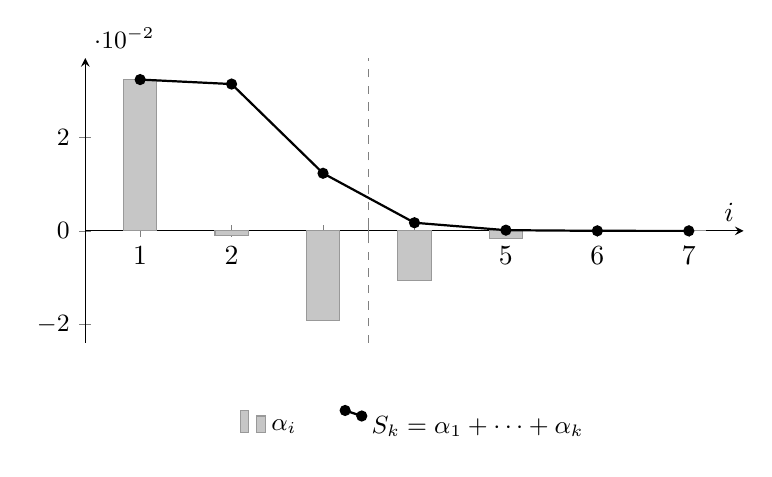
\begin{tikzpicture}
\begin{axis}[width=0.82\textwidth,height=5.2cm,ybar,bar width=12pt,xmin=0.4,xmax=7.6,ymin=-0.024,ymax=0.037,
  xtick={1,...,7},xlabel={$i$},ylabel={},axis x line=middle,axis y line=left,
  legend style={at={(0.5,-0.2)},anchor=north,draw=none,font=\small,legend columns=2,/tikz/every even column/.append style={column sep=14pt}},
  yticklabel style={/pgf/number format/fixed,/pgf/number format/precision=2,font=\small},
  extra x ticks={3.5},extra x tick labels={},extra x tick style={grid=major,major grid style={dashed,gray}}]
\addplot[fill=gray!45,draw=gray!80] coordinates {(1,0.0323935) (2,-0.00095999) (3,-0.0191015) (4,-0.0105921)
  (5,-0.00159039) (6,-0.000143686) (7,-0.0000059)};
\addlegendentry{$\alpha_i$}
\addplot[sharp plot,mark=*,mark size=1.6pt,thick,black] coordinates {(1,0.0323935) (2,0.0314335) (3,0.0123321)
  (4,0.00173998) (5,0.000149591) (6,0.0000059) (7,0)};
\addlegendentry{$S_k=\alpha_1+\dots+\alpha_k$}
\end{axis}
\end{tikzpicture}
\caption{$X\sim\Bin(10,3/10)$. The bars are $\alpha_i$, continued past $i=m=3$ (dashed line) up to $i=n-m=7$; the dots
are the partial sums. The bars fall and then rise, end below zero, and add up to zero, so the partial sums rise, then
fall, and reach zero only at the end. The conjecture concerns $k\le3$.}
\label{fig:alpha}
\end{figure}

The argument is a general lemma about integer-valued variables (Section~\ref{sec:lemma}) plus one identity for the
binomial (Section~\ref{sec:binomial}). Two ingredients are already in \cite{FPP}: the sum identity behind
Lemma~\ref{lem:sum} is a form of their Lemma~2.1, and comparing $\Prob(X=m+i)$ with $\Prob(X=m-i)$ through their ratio
is how they treat the Poisson case \cite[Lemma~3.6]{FPP}. What is added here is continuing the index past $m$, which
turns the sign pattern of these ratios into nonnegativity of every partial sum, with strict positivity for the
binomial when $n>2m$ and $1\le k<n-m$. The lemma then gives short proofs for the
Poisson distribution, recovering \cite[Lemma 3.7]{FPP}, and for the negative binomial distributions $\NB(r,1-1/n)$, for which the authors observed
that left-loadedness ``appears to be true'' \cite[p.~140]{FPP} (Section~\ref{sec:other}).

\section{A lemma on reflected differences}\label{sec:lemma}

Let $X$ take values in the nonnegative integers, with finite mean equal to an integer $m\ge1$. Write $p_j=\Prob(X=j)$,
with $p_j=0$ for $j<0$, and define for every $i\ge1$
\[
\alpha_i=\Prob(X\le m-i)-\Prob(X\ge m+i),\qquad d_i=p_{m+i}-p_{m-i}.
\]
So $\alpha_i$ compares the two tails at distance $i$ from the mean, and $d_i$ compares the two single values at that
distance. The tails lose those values as $i$ grows, which gives
\begin{equation}\label{eq:step}
\alpha_{i+1}-\alpha_i=d_i\qquad(i\ge1).
\end{equation}

\begin{lem}\label{lem:sum}
$\sum_{i\ge1}\alpha_i=0$, the series converging absolutely, and $\alpha_i\to0$.
\end{lem}

\begin{proof}
Counting each value $j$ once for every $i$ it is counted in, $\sum_{i\ge1}\Prob(X\le m-i)=\sum_j (m-j)^+p_j=\E(m-X)^+$
and $\sum_{i\ge1}\Prob(X\ge m+i)=\E(X-m)^+$, both finite. Their difference is $\E(m-X)=0$. (Fokkink,
Papavassiliou and Pelekis use the same counting to show $\alpha_1+\dots+\alpha_m=\sum_{i>m}\Prob(X\ge m+i)$
\cite[Lemma~2.1]{FPP}.)
\end{proof}

\begin{lem}\label{lem:main}
Suppose there is an index $r\ge1$ with $d_i\le0$ for $1\le i<r$ and $d_i\ge0$ for $i\ge r$. Then there is an $\ell\ge0$
with $\alpha_i\ge0$ for $i\le\ell$ and $\alpha_i\le0$ for $i>\ell$, and every partial sum $S_k=\alpha_1+\dots+\alpha_k$
is nonnegative. In particular $X$ is left-loaded.
\end{lem}

\begin{proof}
By \eqref{eq:step}, $\alpha_1\ge\alpha_2\ge\dots\ge\alpha_r$ and $\alpha_r\le\alpha_{r+1}\le\cdots$. The second run is
nondecreasing with limit $0$ (Lemma~\ref{lem:sum}), so all its terms are at most $0$. The first run is nonincreasing,
so its nonnegative terms come first. Let $\ell=\max\bigl(\{0\}\cup\{i\le r:\alpha_i\ge0\}\bigr)$, a finite
number. Then $\alpha_i\ge0$ for $i\le\ell$ and $\alpha_i\le0$ for $i>\ell$, so $S_k\ge0$ for $k\le\ell$, and for
$k>\ell$ we have $S_k=-\sum_{i>k}\alpha_i\ge0$ by Lemma~\ref{lem:sum}.
\end{proof}

Read in words: if the probability mass above the mean overtakes its mirror image below the mean only once, the lower
tail wins near the mean and loses further out, and the total bookkeeping of the integer mean keeps every partial sum on
the right side of zero.

\section{The binomial distribution}\label{sec:binomial}

Let $X\sim\Bin(n,m/n)$ and $q=n-m$. If $q=m$ the distribution is symmetric about $m$ and every $\alpha_i$ vanishes, so
assume $q>m$. Consecutive probabilities satisfy $p_{j+1}/p_j=\frac{(n-j)m}{(j+1)q}$. For $0\le i\le m$ put
$\beta_i=p_{m+i}/p_{m-i}$, the ratio of a value above the mean to its mirror image, so that $\beta_0=1$ and
$d_i=p_{m-i}(\beta_i-1)$.

\begin{lem}\label{lem:ratio}
For $0\le i\le m-1$,
\[
\frac{\beta_{i+1}}{\beta_i}-1=\frac{(q-m)\bigl((q+m)\,i(i+1)-mq\bigr)}{q^2(m-i)(m+i+1)}.
\]
\end{lem}

\begin{proof}
From the ratio of consecutive probabilities,
\[
\frac{\beta_{i+1}}{\beta_i}=\frac{p_{m+i+1}}{p_{m+i}}\cdot\frac{p_{m-i}}{p_{m-i-1}}
=\frac{(q-i)m}{(m+i+1)q}\cdot\frac{(q+i+1)m}{(m-i)q}=\frac{m^2(q-i)(q+i+1)}{q^2(m-i)(m+i+1)}.
\]
Write $t=i(i+1)$. Then $(q-i)(q+i+1)=q(q+1)-t$ and $(m-i)(m+i+1)=m(m+1)-t$, and
$m^2\bigl(q(q+1)-t\bigr)-q^2\bigl(m(m+1)-t\bigr)=mq(m-q)+(q^2-m^2)t=(q-m)\bigl((q+m)t-mq\bigr)$.
\end{proof}

The factor $(q+m)i(i+1)-mq$ is increasing in $i$ and equals $-mq<0$ at $i=0$. So $\beta_{i+1}/\beta_i$ is below $1$
for small $i$ and at least $1$ from some point on: the ratios $\beta_i$ first decrease from $\beta_0=1$ and then
increase. In particular $\beta_i<1$ for $1\le i\le r'$ and $\beta_i\ge1$ for $r'<i\le m$, for some $r'$. Hence
$d_i<0$ for $1\le i\le r'$ and $d_i\ge0$ for $r'<i\le m$, and $d_i=p_{m+i}>0$ for $m<i\le q$ because $p_{m-i}=0$
there.

\begin{proof}[Proof of Theorem~\ref{thm:main}]
Lemma~\ref{lem:main} applies with $r=r'+1$. Since $X\le n$, $\alpha_i=0$ for $i>q$, and
$\alpha_q=\Prob(X\le m-q)-\Prob(X\ge n)=-p_n<0$. The proof of Lemma~\ref{lem:main} shows that $(\alpha_i)$ is
nonnegative up to $\ell$ and nonpositive after, and $\ell<q$ because $\alpha_q<0$; the negative terms after $\ell$ are
strictly negative, since a zero term in the nondecreasing run would force all later terms up to $q$ to vanish. If
$\alpha_1\le0$, all of $\alpha_1,\dots,\alpha_q$ would be at most $0$ with $\alpha_q<0$, contradicting
$\sum_{i\le q}\alpha_i=0$; hence $\alpha_1>0$, which is \eqref{eq:simmons}. So $S_k\ge\alpha_1>0$ for $k\le\ell$, and
for $\ell\le k<q$ we have $S_k=-(\alpha_{k+1}+\dots+\alpha_q)>0$. As $m<q$, this covers $1\le k\le m$, and the sign
pattern on $\alpha_1,\dots,\alpha_m$ is the restriction of the one on $\alpha_1,\dots,\alpha_q$.
\end{proof}

The positivity can be very tight. For $k=m$ the partial sum is $S_m=\sum_{i>m}\Prob(X\ge m+i)$, which for $n=2m+1$ is
$\Prob(X=n)=(m/n)^n$.

\section{Other distributions}\label{sec:other}

\begin{prop}\label{prop:poisson}
A Poisson variable with integer mean $m\ge1$ is left-loaded.
\end{prop}

\begin{proof}
Here $p_{j+1}/p_j=m/(j+1)$, so for $0\le i\le m-1$ the ratio $\beta_i=p_{m+i}/p_{m-i}$ satisfies
$\beta_{i+1}/\beta_i=m^2/\bigl((m-i)(m+i+1)\bigr)$, which is at least $1$ exactly when $i(i+1)\ge m$. As in
Section~\ref{sec:binomial}, $\beta$ decreases from $\beta_0=1$ and then increases, so $d_i$ is negative and then
nonnegative for $i\le m$, and $d_i=p_{m+i}>0$ for $i>m$. Lemma~\ref{lem:main} applies.
\end{proof}

This is \cite[Lemma 3.7]{FPP}. The ratio computation is theirs \cite[Lemma~3.6]{FPP}; their proof then needs the
inequality $\Prob(X\ge2m)>\Prob(X=0)$ for $m\ge3$ \cite[Lemma~3.5]{FPP} and treats $m\in\{1,2\}$ separately,
and continuing past $m$ makes both unnecessary.

\begin{prop}\label{prop:nb}
Let $n\ge2$ and $r\ge1$ be integers and $X\sim\NB(r,1-1/n)$, the number of successes before the $r$-th failure when
each trial succeeds with probability $1-1/n$. Then $X$ has integer mean $m=r(n-1)$ and is left-loaded.
\end{prop}

\begin{proof}
Write $\pi=1-1/n$. The mean is $r\pi/(1-\pi)=r(n-1)$ and $p_{j+1}/p_j=(j+r)\pi/(j+1)$. For $0\le i\le m-1$,
\[
\frac{\beta_{i+1}}{\beta_i}=\frac{(m+i+r)\pi}{m+i+1}\cdot\frac{(m-i+r-1)\pi}{m-i},\qquad
\frac{\beta_{i+1}}{\beta_i}-1=\frac{(2n-1)\bigl(i(i+1)-mn\bigr)}{n^2(m-i)(m+i+1)},
\]
the second by substituting $\pi=(n-1)/n$ and $m+r=rn$. The factor $i(i+1)-mn$ is increasing and negative at $i=0$,
so as for the binomial, $\beta$ decreases from $\beta_0=1$ and then increases, $d_i$ is negative and then nonnegative
for $i\le m$, and $d_i=p_{m+i}>0$ for $i>m$. Lemma~\ref{lem:main} applies.
\end{proof}

Fokkink, Papavassiliou and Pelekis show that these negative binomial distributions are right-skewed
\cite[Lemma 3.3]{FPP} and remark that left-loadedness appears to hold too; Proposition~\ref{prop:nb} confirms it.

\begin{cor}\label{cor:tails}
Let $N,s$ be positive integers, $S\sim\Bin(N,s/N)$ with $N\ge2s$, and let $X$, independent of $S$, be $\Bin(n,m/n)$ with $n\ge2m$, or
$\Poi(m)$, or $\NB(r,1-1/n)$ with mean $m=r(n-1)$. If $s\ge m\ge1$, then $\Prob(S\ge s)\ge\Prob(S+X\ge s+m)$.
\end{cor}

\begin{proof}
$S$ is right-skewed with mode $s$ \cite[Lemma 3.2]{FPP} and $X$ is left-loaded with mean $m$ (Theorem~\ref{thm:main},
Propositions~\ref{prop:poisson} and \ref{prop:nb}), so \cite[Theorem 1.1]{FPP} applies.
\end{proof}

\noindent The Poisson case of Corollary~\ref{cor:tails} is stated in \cite{FPP}, and \cite[p.~140]{FPP} indicates
the binomial case for some ranges of $m$; Theorem~\ref{thm:main} and Proposition~\ref{prop:nb} give the rest. Corollary~\ref{cor:tails} with $S\sim\Bin(nk,m/n)$ and $X\sim\Bin(n,m/n)$, $n>2m$, gives back the
monotonicity $\Prob(\Bin(nk,m/n)\ge km)\ge\Prob(\Bin(n(k+1),m/n)\ge(k+1)m)$, which Jogdeo and Samuels proved for all
$n\ge m$ \cite{JS}; the point of Corollary~\ref{cor:tails} is that $S$ and $X$ may have different parameters.

\section{Data, code and the use of AI tools}\sloppy

The exact computations (rational arithmetic, all $n\le400$ for the binomial, and the negative binomial for $r\le6$,
$n\le7$), the checks of every identity, and the Lean files are in the folder \texttt{simmons-left-loaded} of
\href{https://github.com/jvvk/mathematics}{github.com/jvvk/mathematics} and archived on Zenodo.

Theorem~\ref{thm:main} is formalised in Lean~4 with Mathlib, in integer arithmetic (the probabilities multiplied by
$n^n$, with a separate proof that these integers divided by $n^n$ are the binomial probabilities): the step identity
\eqref{eq:step}, the zero sum, the value $\alpha_q=-p_n$, Lemma~\ref{lem:ratio}, the sign pattern, the positivity
of $S_k$ for $1\le k<n-m$ and the case $n=2m$. The proofs use only Lean's standard axioms, and fourteen false
strengthenings of the formal statements are each rejected. Lemma~\ref{lem:main} in its general form and
Section~\ref{sec:other} are not formalised. The programs check the ratio identities of Lemma~\ref{lem:ratio} and
Propositions~\ref{prop:poisson} and~\ref{prop:nb} symbolically, the binomial statement exactly for every $n\le400$,
and the negative binomial partial sums exactly for $r\le6$, $n\le7$; they do not check Lemma~\ref{lem:main} in
general, the Poisson partial sums or Corollary~\ref{cor:tails}, which rest on the proofs above.

The author used AI tools. Codex (OpenAI) found the proof of Theorem~\ref{thm:main}, extending $\alpha$ past $m$.
Claude (Anthropic) checked it, found the general form of Lemma~\ref{lem:main} and Propositions~\ref{prop:poisson}
and~\ref{prop:nb}, wrote the Lean formalisation and the text. The author is responsible for the content.

\begin{thebibliography}{9}
\bibitem{FPP} R.~Fokkink, S.~Papavassiliou and C.~Pelekis, On the monotonicity of tail probabilities,
\emph{Probab. Math. Statist.} \textbf{42} (2022), 133--141, \doi{10.37190/0208-4147.00050}.
\bibitem{JS} K.~Jogdeo and S.~M.~Samuels, Monotone convergence of binomial probabilities and a generalization of
Ramanujan's equation, \emph{Ann. Math. Statist.} \textbf{39} (1968), 1191--1195, \doi{10.1214/aoms/1177698243}.
\bibitem{MO} Simmons' inequality on binomial random variables, MathOverflow question 384456 (2021),
\url{https://mathoverflow.net/q/384456}, accessed 24 November 2026.
\bibitem{PR} O.~Perrin and E.~Redside, Generalization of Simmons' theorem, \emph{Statist. Probab. Lett.} \textbf{77}
(2007), 604--606, \doi{10.1016/j.spl.2006.09.006}.
\bibitem{Simmons} T.~C.~Simmons, A new theorem in probability, \emph{Proc. London Math. Soc.} \textbf{s1-26} (1894),
290--325, \doi{10.1112/plms/s1-26.1.290}.
\end{thebibliography}

\end{document}
